\chapter{Grundlagen}
\label{cha:fundamentals}

Im Kapitel Grundlagen werden die erfordentlichen Grundlagen erläutert, die notwendig sind, um die Funktionsweise von Style Transfer zu verstehen. Außerdem wird auf bestehende Arbeiten in diesem Bereich eingegangen.

\section{Feedforward Neural Network}

Feedforward Neural Networks werden im Bereich des Deep Learning eingesetzt. Dabei werden unterschiedliche Arten von Layern zu einem Neuronalen Netzwerk zusammen gesetzt. Je nach Aufgabenstellung sind verschiedene Arten von Layer-Kombinationen sinnvoll.

Ein Feedforward Neural Network definiert eine Abildung von $ y = f(x; \phi) $, wobei $ \phi $ (auch mit $ w $ notiert) Gewichtungsparameter des Netzwerks sind. Es wird Feedforward genannt, da die Informationen $ x $ von vorne nach hinten durch die einzelnen Layer des Netwerks fließen und am Ende $ y $ ausgeben. Die Layer des Netzwerks sind dabei wiederum Unterfunktionen die in einer Kettenstruktur ineinander übergehen. Bei einem Neuronalen Netzwerk mit den drei Layern $ f^{(1)} $, $ f^{(2)} $, $ f^{(2)} $ ergibt sich der Aufbau $ f(x) = f^{(3)}(f^{(2)}(f^{(1)}(x))) $. Der erste Layer eines Netzwerks nennt sich Input-Layer, der letzte Output-Layer. Alle zwischenliegenden Layer werden Hidden-Layer genannt. Je mehr Layer ein Netzwerk besitzt, desto komplexere mathematische Funktionen kann es abbilden und desto tiefer ist es. Daher rührt auch der Name Deep Neural Network und Deep Learning \cite[164-165]{Goodfellow-et-al-2016}.

\pagebreak

\section{Fully-Connected Neural Network}

Fully-Connected Neural Networks bestehen aus mehreren hintereinander geschalteten Fully-Connected-Layern. Der Name rührt daher, dass zwischen zwei aufeinanderfolgenden Layern alle Neuronen miteinander verbunden sind.

\begin{figure}[H]
	\centering
	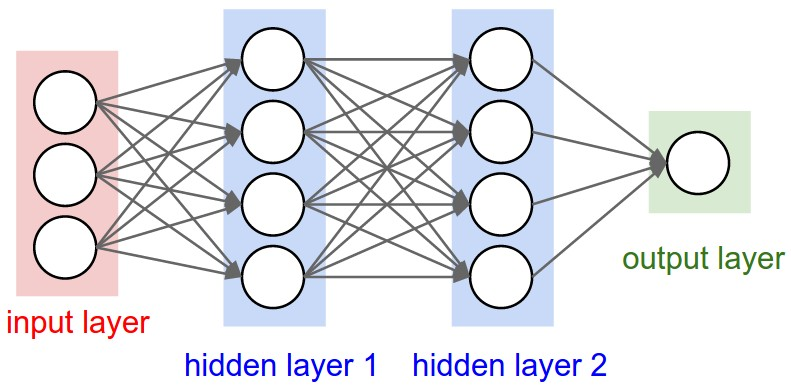
\includegraphics[width=0.95\textwidth]{resources/content/fully_connected.jpg}
	\caption{Fully-Connected Neural Network \cite{fully_connected_img}}
	\label{img:fully_connected}
\end{figure}

Die Kreise stellen die Neuronen dar und die Kanten sind die Gewichtungsfaktoren.
Eine solche Struktur kann mit einer einzigen Matrix-Multiplikation berechnet werden.

\begin{align}
	f(x) = \sigma(x * w + b)
\end{align}

In der Formel steht $ x $ für die Eingangsdaten, $ w $ für die Gewichtungsfaktoren, $ b $ für einen Biaswert. Letztlich läuft das berechnete Ergebniss durch eine Aktivierungsfunktion $ \sigma $, die nachfolgend in \ref{sec:activation_functions} beschrieben wird.

Ausgehend von einem Neuronalen Netzwerk mit einem Input-Layer mit zwei Neuronen, einem Hidden-Layer mit drei Neuronen, einem Output-Layer mit einem Neuron, einer Minibatchgröße von drei und der Aktvierungsfunktion $ \sigma(x) = {\begin{cases}0&{\text{if }}x<0\\x&{\text{if }}x\geq 0\end{cases}} $ ergibt sich folgendes Beispiel:

\begin{equation}
	\vspace{5pt}
	x = \begin{pmatrix} 
		0.0 & 0.0 \\
		1.0 & 1.0 \\ 
		2.0 & 2.0
	\end{pmatrix}
	\vspace{5pt}
	w_{1} = \begin{pmatrix} 
		1.0 & 1.0 \\
		1.0 & 1.0 \\ 
		0.5 & 0.5
	\end{pmatrix}
	\vspace{5pt}
	w_{2} = \begin{pmatrix} 
		1.0 \\
		1.0 \\ 
		0.5
	\end{pmatrix}
\end{equation}

Die Werte der letzten Zeilen in den Gewichtsmatrizen $ w_{1} $ und $ w_{2} $ sind die Gewichtungsfaktoren für den Bias-Wert. Den Eingabedaten $ x $ wird vor Durchlauf durch einen Layer ein fester Wert (Bias) von $ 1 $ hinzugefügt. Nach Durchlauf durch den ersten Layer ergibt sich dementsprechend folgendes Zwischenergebnis:

\begin{equation}
	\sigma \left(
	\begin{pmatrix} 
		0.0 & 0.0 & 1.0 \\
		1.0 & 1.0 & 1.0 \\ 
		2.0 & 2.0 & 1.0
	\end{pmatrix} 
	\times
	\begin{pmatrix} 
		1.0 & 1.0 \\
		1.0 & 1.0 \\ 
		0.5 & 0.5
	\end{pmatrix}
	\right)
	= 
	\begin{pmatrix} 
		0.5 & 0.5 \\
		2.5 & 2.5 \\ 
		4.5 & 4.5
	\end{pmatrix}
\end{equation}

Wiederholt wird dieser Vorgang mit der Gewichtsmatrix $ w_{2} $ des zweiten Layers:

\begin{equation}
	\sigma \left(
	\begin{pmatrix} 
		0.5 & 0.5 & 1.0 \\
		2.5 & 2.5 & 1.0 \\ 
		4.5 & 4.5 & 1.0
	\end{pmatrix}
	\times
	\begin{pmatrix} 
		1.0 \\
		1.0 \\ 
		0.5
	\end{pmatrix}
	\right)
	= 
	\begin{pmatrix} 
		1.5 \\
		5.5 \\ 
		9.5
	\end{pmatrix}
\end{equation}

\section{Aktivierungsfunktionen}
\label{sec:activation_functions}

Die im voherigen Beispiel verwendete Aktivierungsfunktion nennt sich ReLU \cite{Nair:2010:RLU:3104322.3104425}.

\begin{figure}[H]
	\centering
	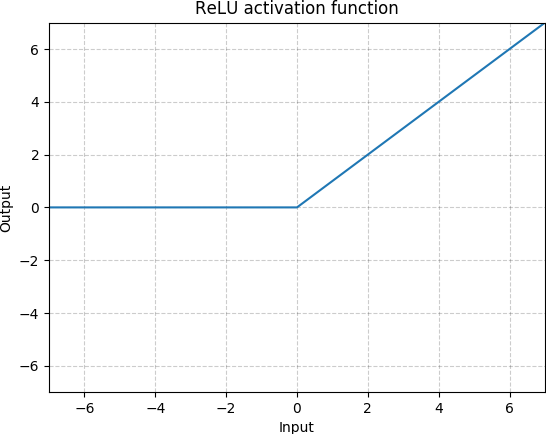
\includegraphics[width=0.50\textwidth]{resources/content/ReLU.png}
	\caption{ReLU-Aktivierungsfunktion \cite{relu_activation_function_img}}
	\label{img:relu_activation_function}
\end{figure}


Neben der ReLU-Aktivierungsfunktion existieren weitere Aktiverungsfunktionen, die im Zusammenhang mit Neuronalen Netzwerken verwendet werden.
Im Folgenden werden die in dieser Arbeit verwendeten Aktivierungsfunktionen beschrieben.

\subsection{LeakyReLU, PReLU}

Die Aktiverungsfunktionen LeakyReLU und PReLU sind Abwandlungen von ReLU und werden um den Parameter $ \alpha $ ergänzt. Bei LeakyReLU handelt es sich bei $ \alpha $ um einen fixen, einstellbaren Wert und bei PReLU wird dieser im Laufe der Trainingsphase gelernt \cite{DBLP:journals/corr/XuWCL15}. ReLU hat gegenüber PReLU und LeakyReLU den Nachteil, dass Neuronen deaktiviert werden können, da die linke Seite der Aktiverungsfunktion 0 beträgt. Somit ergeben sich auch bei der Berechnung der Gradienten keine Veränderungen.

\begin{equation}
	\sigma(\alpha ,x) = {
		\begin{cases}
			\alpha x & {\text{if }} x < 0 \\
			x        & {\text{if }} x \geq 0
		\end{cases}
	}
\end{equation}

Visualisiert besitzen beide Aktiverungsfunktionen folgende Form:

\begin{figure}[H]
	\centering
	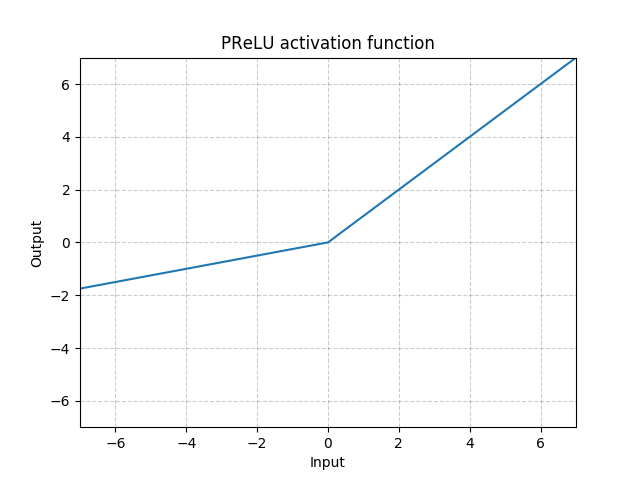
\includegraphics[width=0.50\textwidth]{resources/content/PReLU.png}
	\caption{LeakyReLU-, PReLU-Aktivierungsfunktion \cite{prelu_activation_function_img}}
	\label{img:prelu_activation_function}
\end{figure}

\subsection{Hardtanh}
\label{sec:hardtanh}

Die Hardtanh Funktion wird in dieser Arbeit als abschließende Aktiverungsfunktion genutzt \cite{DBLP:journals/corr/abs-1811-03378, Collobert:2011:NLP:1953048.2078186}.

\begin{equation}
	\sigma(x) = {
		\begin{cases}
			1  & {\text{if }} x > 1 \\ 
			-1 & {\text{if }} x < -1 \\
			x  & {\text{otherwise}}
		\end{cases}
	 }
\end{equation}

\pagebreak

Sie ist in der Lage die Ergebnisse auf einen festgelegten Bereich zu beschränken.

\begin{figure}[H]
	\centering
	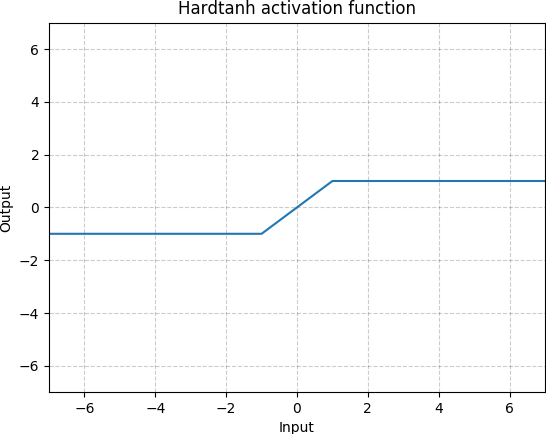
\includegraphics[width=0.55\textwidth]{resources/content/Hardtanh.png}
	\caption{Hardtanh-Aktivierungsfunktion \cite{hardtanh_activation_function_img}}
	\label{img:hardtanh_activation_function}
\end{figure}

\subsection{Sigmoid}
\label{sec:sigmoid}

Die Sigmoid-Funktion wird in dieser Arbeit als alternative, abschließende Aktivierungsfunktion genutzt \cite{DBLP:journals/corr/abs-1811-03378}.

\begin{equation}
	\sigma(x) = \frac{ 1 } { 
		1 + e^{ -x }
	}
\end{equation}

Die Ergebnisse der Sigmoid-Funktion konvergieren zu 0 und 1, ereichen diese jedoch nie komplett.

\begin{figure}[H]
	\centering
	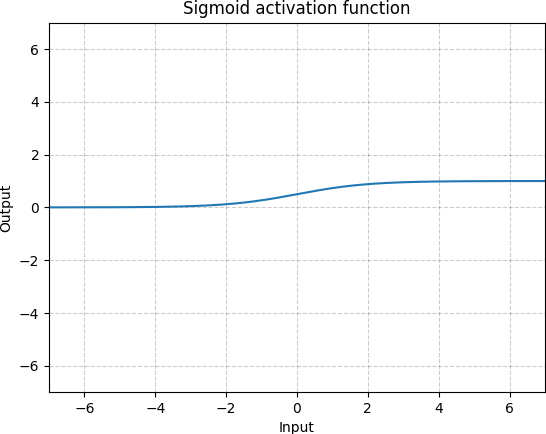
\includegraphics[width=0.55\textwidth]{resources/content/Sigmoid.png}
	\caption{Sigmoid-Aktivierungsfunktion \cite{sigmoid_activation_function_img}}
	\label{img:sigmoid_activation_function}
\end{figure}

\section{Convolutional Neural Network}
\label{sec:conv_networks}

Ein Convolutional Neural Network, auch CNN genannt, besteht aus mehreren aufeinanderfolgenden Convolutional-Layern sowie
abschließend beliebig vielen Fully-Connected-Layern (siehe \ref{img:cnn_example_network}). Convolutional-Layer dienen der Featureextraktion. Die Fully-Connected-Layer sind für die Klassifizierung zuständig. Nachfolgend wird das Prinzip einer Convolution (zu dt. Faltung) erläutert.

\begin{figure}[H]
	\centering
	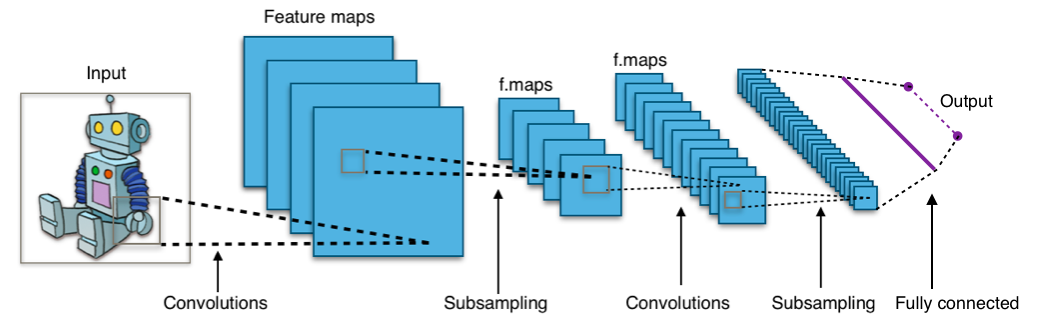
\includegraphics[width=0.95\textwidth]{resources/content/cnn/typical_cnn.png}
	\caption{Beispiel CNN Architektur \cite{typical_cnn_img}}
	\label{img:cnn_example_network}
\end{figure}

Ein Convolutional-Layer akzeptiert Daten in Form eines Bildes $ I $ in den Dimensionen $ W_1 \times H_1 \times C_1 $. Optional wird das Bild mit $ P $ Nullen an den Rändern aufgefüllt. Über das Bild fahren $ N $ Filter der Größe $ F $ mit einer Schrittweite $ S $ und führen an jeder Stelle ein Skalarprodukt mit den Daten der Bildmatrix durch. Daraus ergibt sich eine neue Matrix mit den Dimensionen $ W_2 \times H_2 \times C_2 $:

\begin{itemize}
	\item $ W_2 = (W_1 - F) / S + 1 $
	\item $ H_2 = (H_1 - F) / S + 1 $
	\item $ C_2 = N $
\end{itemize}

\begin{figure}[H]
	\centering
	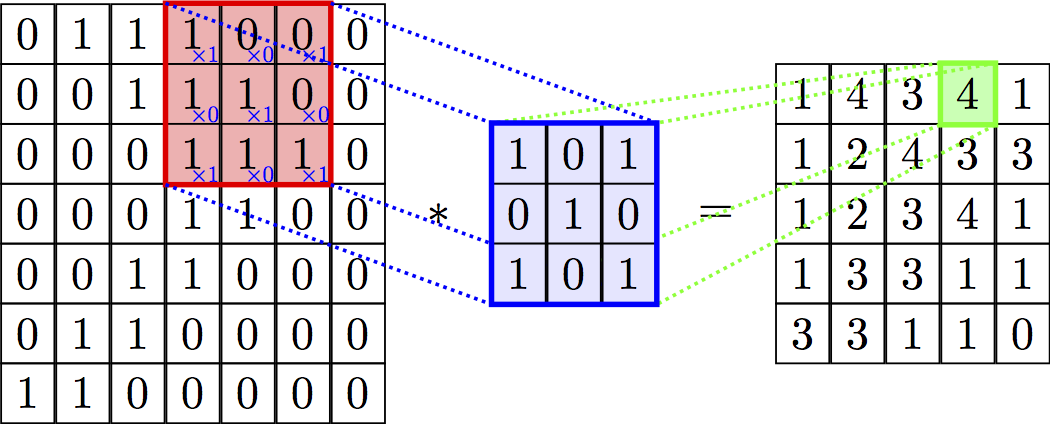
\includegraphics[width=0.90\textwidth]{resources/content/cnn/convolution_croped.png}
	\caption{Berechnungsschritt während einer Convolution \cite{convolution_img}}
	\label{img:convolution_img}
\end{figure}

Die Ergebnisse nach Durchlauf eines Convolutional-Layer werden Feature Maps oder \gls{activation_map}s genannt. Im trainierten CNN erkennen frühe Convolutional-Layer Kanten, Kurven und feine Muster. Spätere Layer erkennen komplette geometrische Figuren bis hin zu komplexen Mustern sowie Schemen von realen Objekten und Gegenständen.

\section{Backprogation}
\label{sec:backpropagation}

Um ein Neuronales Netzwerk zu trainieren, muss das Loss, welches durch das Neuronales Netzwerk erzeugt wird, minimiert werden. Dabei berechnet eine Funktion das Loss des Netzwerks. Beispielsweise berechnet sich das \gls{mse_loss} aus der Differenz zwischen $ y $ und $ \hat{y} $, wobei $ y $ die echten gelabelten Ergebnisse sind und $ \hat{y} $ die Vorhersage, die das Neuronale Netzwerk erzeugt.
Anhand dieser Daten kann ein Optimizer, wie beispielsweise \gls{adam} \cite{kingma2015adam}, die Gewichte des Netzwerks anpassen, um das Loss zu minimieren.

\begin{figure}[H]
	\centering
	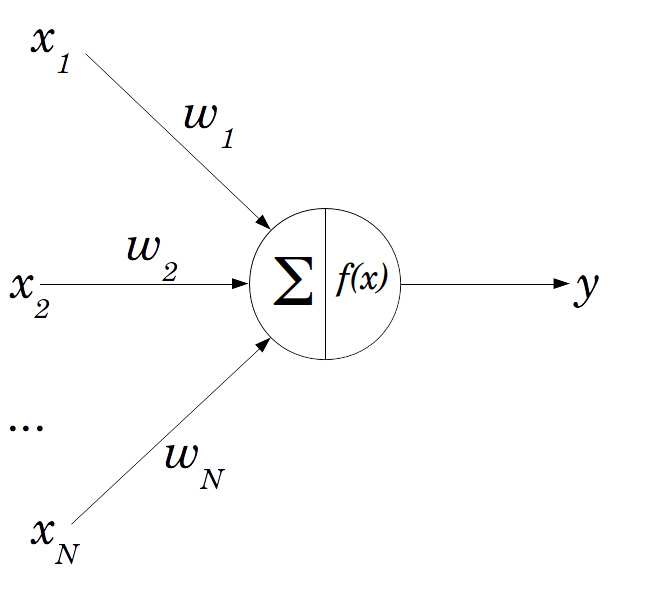
\includegraphics[width=0.4\textwidth]{resources/content/perceptron.png}
	\caption{Visualisierung eines Neurons (auch Perceptron \cite{80230} genannt) \cite{perceptron_img}}
	\label{img:perceptron_img}
\end{figure}

Als Beispiel dient die mathematische Funktion eines 2-dimensionalen Neurons mit angehängter Sigmoid-Aktivierungsfunktion. Dabei werden die Eingabewerte durch die Variable $ x $ und die Gewichte des Neurons durch die Variable $ w $ beschrieben.

\begin{align}
	f(w, x) = \frac{1}{ 1 + e^{ - (w_{0}x_{0} + w_{1}x_{1} + w_{2}) } }
\end{align}

\pagebreak

Folgender Graph veranschaulicht die Berechnung der Gradienten der Funktion.

% https://drive.google.com/file/d/18BC0RLOulbBQSE5Oddg1pVNL9UrhQLx0/view?usp=sharing
\begin{figure}[H]
	\centering
	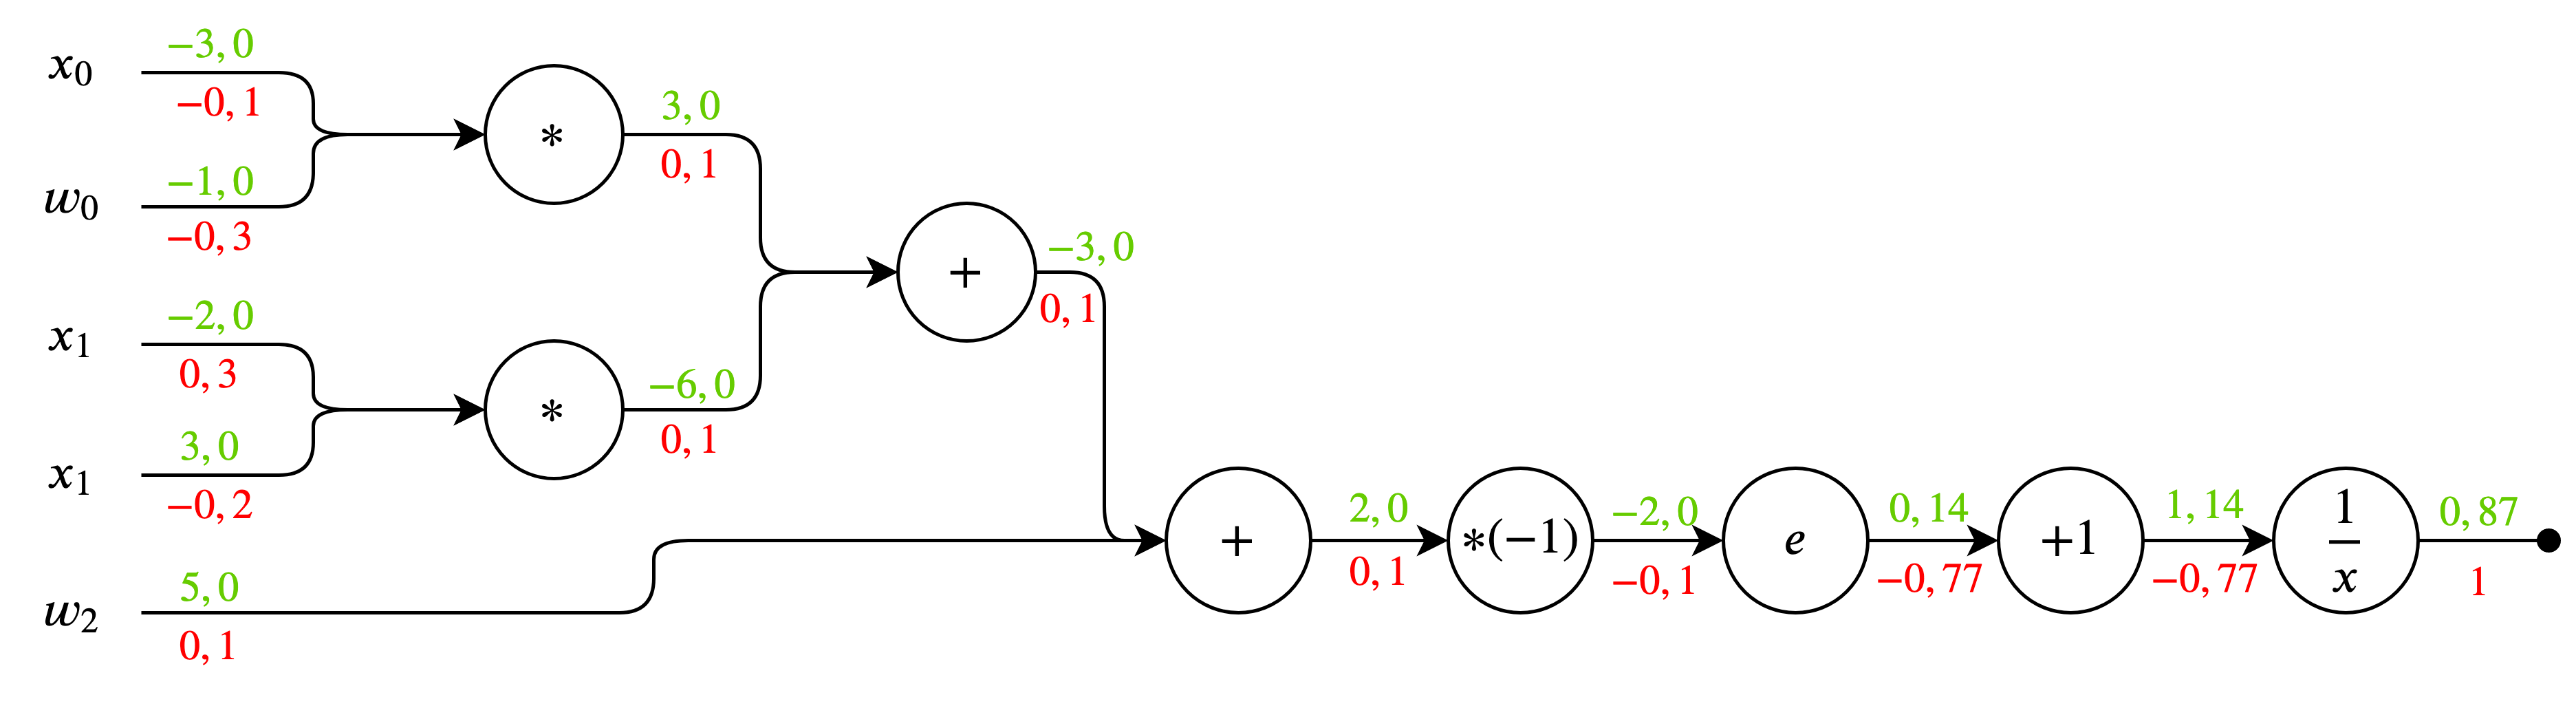
\includegraphics[width=1\textwidth]{resources/content/backpropagation.png}
	\caption{Forward-Pass in Grün und Backward-Pass in Rot dargestellt \cite{cs231n2}}
	\label{img:backpropagation_img}
\end{figure}

Die Funktion wird in beliebig viele Unterfunktionen zerteilt und in Form eines gerichteten Graphen aufgeschrieben.
In einem Forward-Pass werden die Zwischenergebnisse (hier in Grün dargestellt) oberhalb der Kanten festgehalten.

Im Backward-Pass (Zwischenergebnisse in Rot dargestellt) wird von jedem Knoten die erste Ableitung gebildet. Die Zwischenergebnisse des Forward-Pass werden in die Ableitung eingesetzt und danach mit dem Backward-Passergebnis des Folgeschritts multipliziert.

Beispielrechnungen des Backward-Pass der letzten drei Knoten: 

\begin{align}
	& f(x) = \frac{1}{x} \rightarrow \frac{\partial f}{\partial x} = \frac{-1}{ x^{2} }
	& -0,77 \approx 1 * \frac{-1}{ 1,14^{2} }
\end{align}

\begin{align}
	& f(x) = x + 1 \rightarrow \frac{\partial f}{\partial x} = 1
	& -0,77 = -0,77 * 1
\end{align}

\begin{align}
	& f(x) = e^{x} \rightarrow \frac{\partial f}{\partial x} = e^{x}
	& -0,1 \approx -0,77 * e^{-2}
\end{align}

Durch die Berechnung der Gradienten der Gewichtsvariable $ w $ ist der Optimizer in der Lage, $ w $ Schritt für Schritt anzupassen und somit das Loss zu verringern.

\pagebreak

\section{Verwandte Arbeiten}

Diese Arbeit basiert auf den bereits bestehenden Lösungen von Johnson et. al. und Gatys et al., welche in den folgenden Abschnitten erklärt werden.

\subsection{Neural Style Transfer}
\label{sec:neural_style_transfer}

Hierbei handelt es sich um eine Technik um den Stil von artistischen Bildern auf ein anderes willkürliches Bild zu übertragen.
Das Verfahren nutzt dabei einen optimierenden Ansatz. Dabei werden die Pixel eines Eingangsbildes Schritt für Schritt den Pixeln 
des gewünschten Ausgangsbildes angepasst. 

Der Neural Style Transfer Algorithmus, beschrieben im Paper \cite{DBLP:journals/corr/GatysEB15a}, optimiert direkt die Pixel eines Bildes anhand eines sogenannten Perceptual-Loss. Die entsprechende Loss-Funktion besteht aus mehreren Teilen, einem Content-Loss und einem Style-Loss. Optional kann zusätztlich ein Total-Variation-Loss verwendet werden. Das gesamte Perceptual-Loss wird über Hyperparameter konfiguriert, welche die Gewichtung der Unterfunktionen auf das Gesamt-Loss wiederspiegeln.

Content-Loss und Style-Loss benutzen dabei ein bereits auf einem großen Datensatz vortrainiertes Modell. In dieser Arbeit wird das VGG16-Modell \cite{DBLP:journals/corr/SimonyanZ14a} verwendet. Das Content-Loss vergleicht Features eines Inhaltsbildes mit den Features des Ausgangsbild. Das Style-Loss vergleicht Features eines Stilbildes mit den Features des Ausgangsbildes.

\begin{figure}[H]
	\centering
	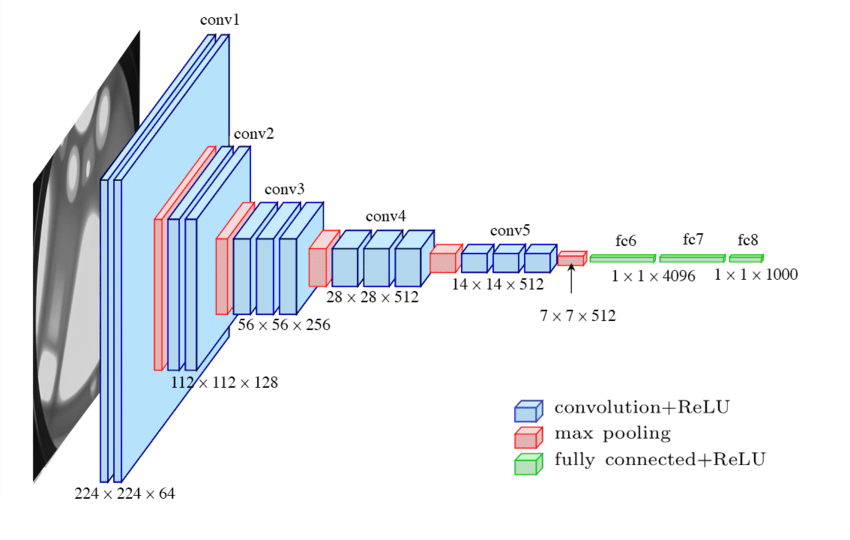
\includegraphics[width=0.70\textwidth]{resources/content/vgg16.png}
	\caption{Architektur des VGG16-Netzwerks \cite{vgg16_img}}
	\label{img:vgg16_img}
\end{figure}

\subsubsection{Content-Loss}
\label{sec:content_loss}

Um das Content-Loss zu berechnen, wird nicht direkt das Contentbild mit dem Ausgangsbild verglichen, stattdessen werden die \gls{activation_map}s nach bestimmten Layern im VGG16-Netzwerk (auch Loss-Network genannt) verwendet. Es ist auch möglich die \gls{activation_map}s mehrerer Layer zu benutzen, da unterschiedliche Layer ein anderes \gls{receptive_field} haben und somit unterschiedliche Informationen speichern.

\begin{figure}[H]
	\centering
	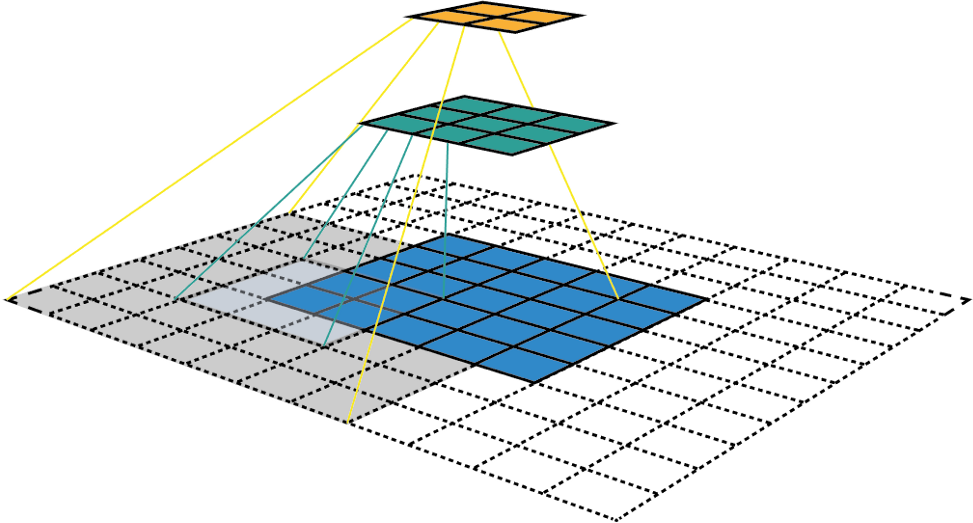
\includegraphics[width=0.79\textwidth]{resources/content/receptive_field.png}
	\caption{Visualisierung des \gls{receptive_field} über drei CNN-Layer \cite{receptive_field_img}}
	\label{img:receptive_field_img}
\end{figure}

Zwischen den \gls{activation_map}s $ P $  des Contentbildes $ \vec{p} $ und den \gls{activation_map}s $ F $ des generierten Bildes $ \vec{x} $ wird das \gls{mse_loss} anhand der gegebenen Layer $ l $ berechnet.

\begin{equation}
	\label{eq:content_loss}
    L_{content} ( \vec{p}, \vec{x}, l ) = \frac{1}{2} \sum_{i, j} (F_{ij}^{l} - P_{ij}^{l})^2
\end{equation}

\subsubsection{Style-Loss}
\label{sec:style_loss}

Das Style-Loss verwendet die \gls{activation_map}s nicht direkt, sondern bildet vorher deren Gram-Matrix. Das hat zur Folge, dass räumliche Informationen verworfen werden, jedoch Farben und Muster erhalten bleiben, die beim Übertragen des Stils die wichtigste Rolle spielen.

Um die Gram-Matrix mehrerer \gls{activation_map}s zu berechnen, werden die Matrizen geflächt und Height- und Width-Dimension werden zu einer Dimension zusammengefügt. Daraus ergibt sich eine 2-dimensionale Matrix der Form $ C \times HW $. Diese wird transponiert mit sich selbst multipliziert.

\begin{equation}
	\label{eq:gram_matrix_1}
	G_{ij}^{l} = \sum_{k} F_{ik}^{l} F_{jk}^{l}
\end{equation}

Es wird die Gram-Matrix, $ G $ aus dem Stilbild und $ A $ aus dem generierten Bild, anhand der gebenen Layer $ l $ berechnet, anschließend normalisiert und das \gls{mse_loss} gebildet.

\begin{equation}
	\label{eq:gram_matrix_2}
	E_{l} = \frac{1}{4N_{l}^{2} M_{l}^2} = \sum_{i, j} ( G_{ij}^{l} - A_{ij}^{l} )^2
\end{equation}

Das Style-Loss ergibt sich aus der gewichteten Summe der Layer-Losses.

\begin{equation}
	\label{eq:style_loss}
	L_{style} ( \vec{a}, \vec{x} ) = \sum_{l=0}^{L} w_{l} E_{l}
\end{equation}

\subsubsection{Total-Variation-Loss}
\label{sec:total_variation_Loss}

Bei der Total-Variation-Loss-Funktion handelt es sich um einen Signal-Denoising-Algorithmus \cite{RUDIN1992259, DBLP:journals/corr/EstrelaMS16}. Sie sorgt dafür das die Pixel der generierten Bilder sanft in einander überlaufen. Farblich sehr unterschiedliche, nah aneinanderliegende Pixel erzeugen ein hohes Loss. So können Verpixelungseffekte vermieden werden. Sie kann optional eingesetzt werden um das Resultat der generierten Bilder zu verbessern.

\begin{equation}
	\label{eq:total_variation_loss}
	L_{tv} ( \vec{x} ) = \sum_{i,j} | y_{i + 1, j} - y_{i, j} | + | y_{i, j + 1} - y_{i,j} |
\end{equation}

\subsubsection{Perceptual-Loss}
\label{sec:perceptual_loss}

Das Perceptual-Loss ist die Kombination aus Content-, Style- und Total-Variation-Loss und wird um die Parameter $ \alpha $, $ \beta $ und $ \gamma $ ergänzt, mit denen die Gewichtung der Losses eingestellt wird.

\begin{equation}
	\label{eq:perceptual_loss}
    L_{perceptual} ( \vec{p}, \vec{a}, \vec{x} ) = \alpha L_{content} ( \vec{p}, \vec{x} ) + \beta L_{style} ( \vec{a}, \vec{x} ) + \gamma L_{tv} ( \vec{x} )
\end{equation}

\subsection{Fast Neural Style Transfer}
\label{sec:fast_neural_style_transfer}

Im Gegensatz zum im Kapitel \ref{sec:neural_style_transfer} vorgestellten Algorithmus, in dem die Pixel des Eingangsbildes direkt optimiert werden, wird ein Neuronales Netzwerk darauf trainiert, die Konzepte eines Stils zu erlernen. Dieses Verfahren wird im Paper \cite{DBLP:journals/corr/JohnsonAL16} genauer beschrieben. Pro Stil wird dabei ein Modell trainiert. Die verwendete Loss-Funktion ist das bereits zuvor beschriebene Perceptual-Loss \ref{sec:perceptual_loss}.

\begin{figure}[H]
	\centering
	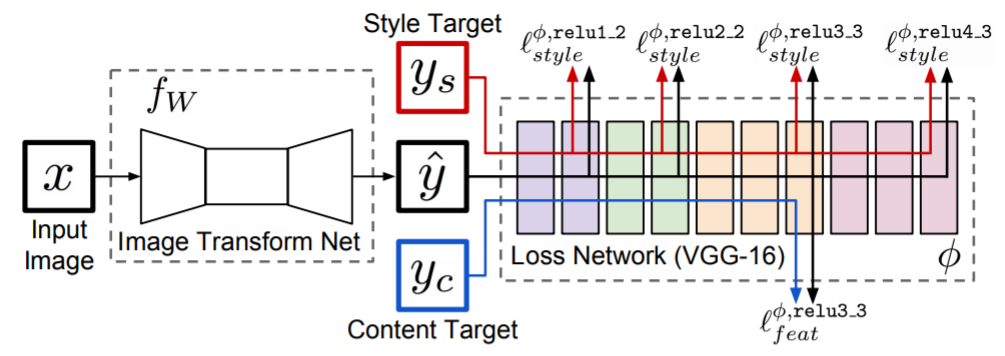
\includegraphics[width=0.79\textwidth]{resources/content/fast_neural_style.png}
	\caption{Trainingsprozess eines Image Transformer Networks \cite{DBLP:journals/corr/JohnsonAL16}}
	\label{img:fast_neural_style_transfer}
\end{figure}

Durch die Verwendung eines Image Transformer Networks kann die Berechnungszeit verbessert werden, da das neu gestylte Bild mit einem Forward-Pass durch das Netzwerk erstellt wird. Die rechenintensive Optimierung und Berechnung der Pixel-Gradienten durch den Backpropagation-Algorithmus \ref{sec:backpropagation} entfällt. Das Training eines Image Transformer Netzworks nimmt jedoch viel Zeit in Anspruch.